%%%%%%%%%%%%%%%%%%%%%%%%%
% Dokumentinformationen %
%%%%%%%%%%%%%%%%%%%%%%%%%
\newcommand{\titleinfo}{Digital Image Processing}
\newcommand{\authorinfo}{R. Koller, L. Schmid} % Do not remove any names! Initial authors stay first.
\newcommand{\versioninfo}{Lectures by Michel Koecher, Markus Thaler}

%%%%%%%%%%%%%%%%%%%%%%%%%%%%%%%%%%%%%%%%%%%%%
% Standard projektïübergreifender Header für
% - Makros 
% - Farben
% - Mathematische Operatoren 
%
% DORT NUR ERGÄNZEN, NICHTS LÖSCHEN
%%%%%%%%%%%%%%%%%%%%%%%%%%%%%%%%%%%%%%%%%%%%%  
% Genereller Header
\documentclass[10pt,twoside,a4paper,fleqn]{article}
\usepackage[left=1cm,right=1cm,top=1cm,bottom=1cm,includeheadfoot]{geometry}
\usepackage[ngerman]{babel,varioref}
\usepackage[utf8]{inputenc}

% Pakete
\usepackage{amssymb}
\usepackage{amsmath}
\usepackage{fancybox}
\usepackage{graphicx}
\usepackage{color}
\usepackage{lastpage}
\usepackage{wrapfig}
\usepackage{fancyhdr}
\usepackage{hyperref}
\usepackage{verbatim}
\usepackage{pdflscape} % landscape
\usepackage{multirow} % zellen in tabellen verbinden
\usepackage{multicol} 
\usepackage{slashbox} % getrennte zelle in tabelle
\usepackage{bm}       % Bold Math

% \usepackage{array} % anordnung in tabellen

%%%%%%%%%%%%%%%%%%%%
% Generelle Makros %
%%%%%%%%%%%%%%%%%%%%
\newcommand{\formelbuch}[1]{$_{\textcolor{red}{\mbox{\small{S#1}}}}$}
\newcommand{\gonzales}[1]{$_{\textcolor{red}{\mbox{\small{Gonzales p #1}}}}$}
\newcommand{\verweis}[2]{ {\small (siehe auch \ref{#1}, #2 (S. \pageref{#1}))
}}
\newcommand{\subsubadd}[1]{\textcolor{black}{\mbox{#1}}}
\newenvironment{liste}[0]{
	\begin{list}{$\bullet$}{\setlength{\itemsep}{0cm}\setlength{\parsep}{0cm} \setlength{\topsep}{0cm}}}
    {\end{list}}
    
\newcommand{\logd}[0]{\log_{10}}
\newcommand{\subsubsubsection}[1]{\textbf{#1}}
\newcommand{\matlab}[1]{\footnotesize{(Matlab: \texttt{#1})}\normalsize{}}

\newenvironment{aufzaehlung}[0]{\begin{enumerate}{\setlength{\itemsep}{0cm}\setlength{\parsep}{0cm}\setlength{\topsep}{0cm}}} {\end{enumerate}}


\newcommand{\abbHeight}[3]{
	\begin{center}
		\includegraphics[height=#2]{./bilder/#1} \\
		#3
    \end{center}
}
\newenvironment{compactList}[0]{
  \begin{list}{$\bullet$}{\setlength{\itemsep}{0cm}\setlength{\parsep}{0cm} \setlength{\topsep}{0cm}}}
    {\end{list}}

\newcommand{\todo}[1]{\colorbox{red}{#1}}
\newcommand{\hilight}[1]{\colorbox{yellow}{#1}}

%\newcommand{\skriptsection}[2]{\section{#1 {\tiny Skript S. #2}}}
%\newcommand{\skriptsubsection}[2]{\subsection{#1 {\tiny Skript S. #2}}}
%\newcommand{\skriptsubsubsection}[2]{\subsubsection{#1 {\tiny Skript S. #2}}}
%\renewcommand{\skriptsection}[2]{\section{#1 {\tiny Schaum S. #2}}}
%\renewcommand{\skriptsubsection}[2]{\subsection{#1 {\tiny Schaum S. #2}}}
%\renewcommand{\skriptsubsubsection}[2]{\subsubsection{#1 {\tiny Schaum S. #2}}}
\newcommand{\skriptsection}[2]{\section{\texorpdfstring{#1 \gonzales{#2}}{#1}}}
\newcommand{\skriptsubsection}[2]{\subsection{\texorpdfstring{#1 \gonzales{#2}}{#1}}}
\newcommand{\skriptsubsubsection}[2]{\subsubsection{\texorpdfstring{#1 \gonzales{#2}}{#1}}}

%%%%%%%%%%
% Farben %
%%%%%%%%%%
\definecolor{black}{rgb}{0,0,0}
\definecolor{red}{rgb}{1,0,0}
\definecolor{white}{rgb}{1,1,1}
\definecolor{grey}{rgb}{0.8,0.8,0.8}

%%%%%%%%%%%%%%%%%%%%%%%%%%%%
% Mathematische Operatoren %
%%%%%%%%%%%%%%%%%%%%%%%%%%%%
\DeclareMathOperator{\sinc}{sinc}
\DeclareMathOperator{\sgn}{sgn}
\DeclareMathOperator{\median}{median}
\DeclareMathOperator{\Lap}{Lap}
\DeclareMathOperator{\ceil}{ceil}



% Fouriertransformationen
\unitlength1cm
\newcommand{\FT}
{
\begin{picture}(1,0.5)
\put(0.2,0.1){\circle{0.14}}\put(0.27,0.1){\line(1,0){0.5}}\put(0.77,0.1){\circle*{0.14}}
\end{picture}
}


\newcommand{\IFT}
{
\begin{picture}(1,0.5)
\put(0.2,0.1){\circle*{0.14}}\put(0.27,0.1){\line(1,0){0.45}}\put(0.77,0.1){\circle{0.14}}
\end{picture}
}



%%%%%%%%%%%%%%%%%%%%%%%%%%%%
% Allgemeine Einstellungen %
%%%%%%%%%%%%%%%%%%%%%%%%%%%%
%pdf info
\hypersetup{pdfauthor={\authorinfo},pdftitle={\titleinfo},colorlinks=false}
\author{\authorinfo}
\title{\titleinfo}

%Kopf- und Fusszeile
\pagestyle{fancy}
\fancyhf{}
%Linien oben und unten
\renewcommand{\headrulewidth}{0.5pt} 
\renewcommand{\footrulewidth}{0.5pt}

\fancyhead[L]{\titleinfo{ }- Summary}
%Kopfzeile rechts bzw. aussen
\fancyhead[R]{\today{ }- Page \thepage/\pageref{LastPage}}
\fancyfoot[C]{\copyright{ }\authorinfo}

% Einr�cken verhindern versuchen
\setlength{\parindent}{0pt}



% Möglichst keine Ergänzungen hier, sondern in header.tex
\begin{document} 
 
%%%%%%%%%%%%%%%%%%%%%%%%%%%%%%%%%%%%%%%%%%%%%%%%%%%%%%%%%%%%%%%%%%%%%%%%%%%%%%%%%%%%%%%%%%%%%%%
%%%%%%%%%%%%%%%%%%%%%%%%%%%%%%%%%%%%%%%%%%%%%%%%%%%%%%%%%%%%%%%%%%%%%%%%%%%%%%%%%%%%%%%%%%%%%%%
\section{Point Operations (V1)}
\begin{tabular}{ll}
  \parbox{8cm}{
    \subsection{Definition}
    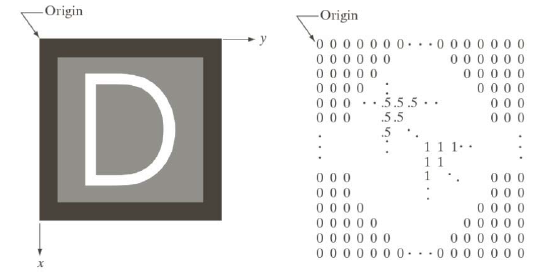
\includegraphics[width=7cm]{./images/image_definition.png}\\
    $M$ rows ($x$) and $N$ columns ($y$)
    } 
  & \parbox{11cm}{
    \subsection{Process}
    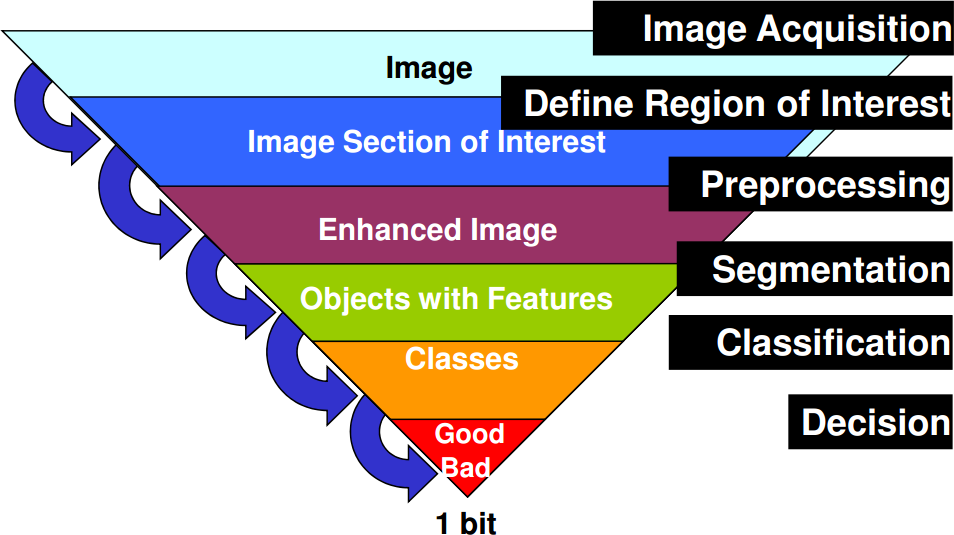
\includegraphics[width=10cm]{./images/image_process.png}
    }
  
\end{tabular}

Homogeneous operations don't depend on coordinates, but inhomogeneous do.



\skriptsubsection{Histogram}{120}

\begin{minipage}{11cm}

  $h(i) = $ number of pixels in $I$ with intensity value $i$\\
  
  Cumulative Histogram (Integral): $H(i) = \sum_{j=0}^i h(j)$ für $0 \leq i \leq K$
  
  Increasing Contrast: $f_c(a) = 1.5 a$\\
  Increasing Brightness: $f_b(a) = a + 10$\\
  Invert Image: $f_i(a) = a_{max} - a$\\

  \textbf{Optimize Dynamic Range} (saturate $s_{low}$\% and $s_{high}$ pixels): \\
  $\hat{a}_{low} = \min\{i | H(i) \geq M \cdot N \cdot s_{low}\}$\\
  $\hat{a}_{high} = \min\{i | H(i) \leq M \cdot N \cdot s_{high}\}$\\
  
  $f_{mac}(a) = \begin{cases}
  a_{min} & \text{ for } a \leq \hat{a}_{low}\\
  a_{min} + (a-a_{low}) \frac{a_{max} - a_{min}}{a_{high} - a_{low}} & \text{ for } \hat{a}_{low} < a < \hat{a}_{high}\\
  a_max & \text{ for } \hat{a}_{high}
  \end{cases}$
  
  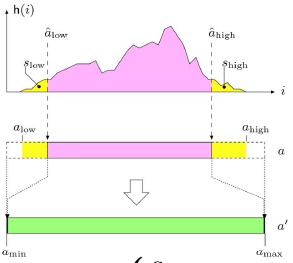
\includegraphics[width=8cm]{./images/automatic_contrast.png}
\end{minipage}
\begin{minipage}{7cm}
  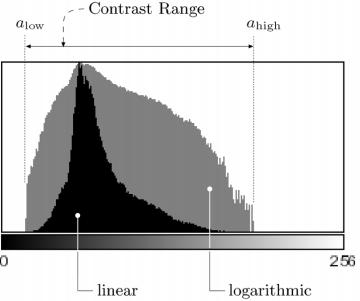
\includegraphics[width=8cm]{./images/contrast.png}

  \textbf{Histogram Equalisation:}\\
  $H(a) = H_{eq}(a')$\\
  $a' = H(a) \frac{255}{M \cdot N}$\\
  $H_{eq}(i) = M \cdot N \cdot i$\\
  $H(a) = a' \frac{M \cdot N}{255} $
  
  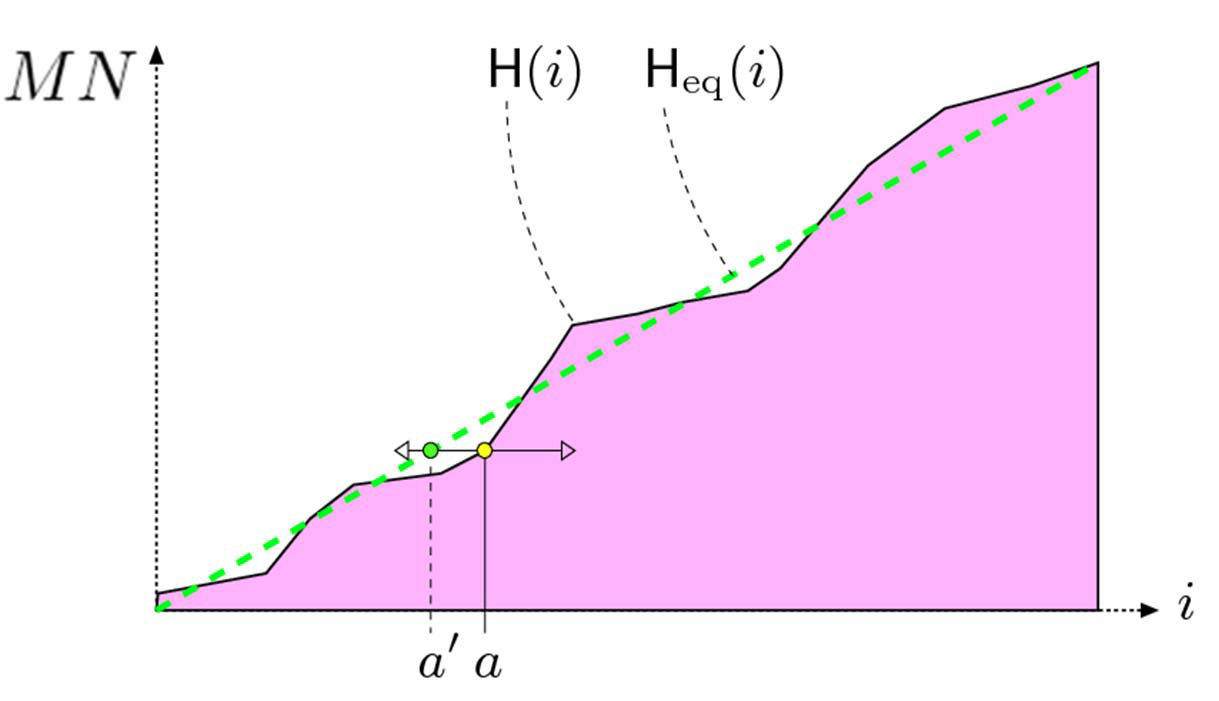
\includegraphics[width=7cm]{./images/histogram_equalisation.png}
\end{minipage}
\clearpage
\skriptsection{Transformations (V2)}{104}
Transformation is done using the inverse transformation $T^{-1}$ which means that the loop is done 
in the output space and not in the input space. Otherwise, some holes or overlaps are possible.

\begin{minipage}{9cm}
  \skriptsubsection{Affine Transformations}{87}
  $[x \; y] = [w \; z] \begin{bmatrix}
  a_{11} &a_{12} \\ a_{21} &a_{22}
  \end{bmatrix} + [b_1 \; b_2]$
  
  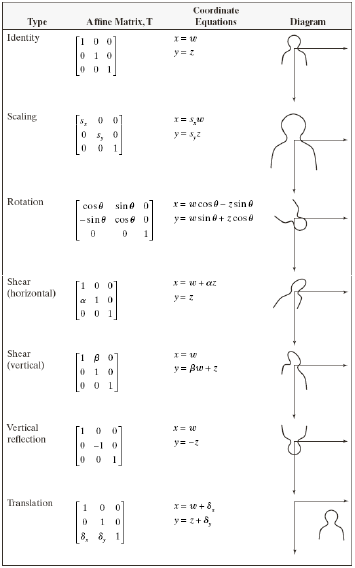
\includegraphics[width=7cm]{./images/affine_transformations.png}
\end{minipage}
\begin{minipage}{9cm}
  \skriptsubsection{Interpolation}{65}
  Methods: Nearest Neighbour; Bilinear (image); Bicubic\\
  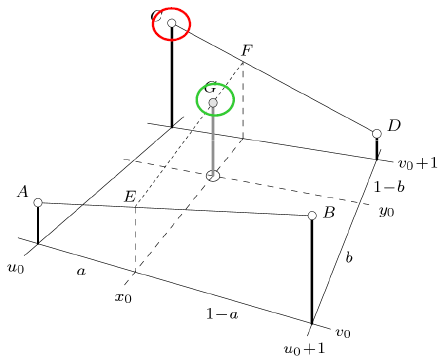
\includegraphics[width=7cm]{./images/bilinear_interpolation.png}
  
  \subsection{Image Registration}
  Image registration is the process of aligning (multiple) images or bringing them into one coordinate 
  system geometrically.
  \begin{itemize}
    \item Feature extraction
    \item Find transform to reference image
    \item Transform image
  \end{itemize}
\end{minipage}


\skriptsection{Filtering in the Spatial Domain (V3)}{144}

\begin{tabular}{ll}
\parbox{7.5cm}{
  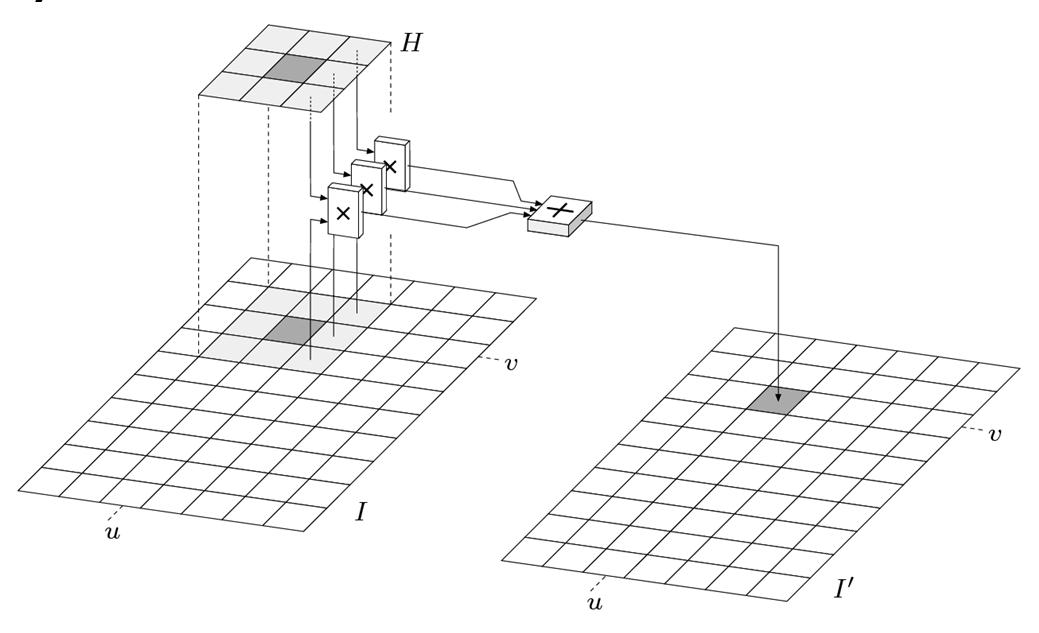
\includegraphics[width=7cm]{./images/filter_matrix.png}}
& \parbox{10cm}{
  Operations on images working with the pixels in the neighbourhood. This is a convolution of image 
  and filter matrix in the spatial domain.
  $$I' = I \ast H$$
  If H is 3x3 matrix and the origin is the center position:
  $$I' = \sum_{i=-1}^{1} \sum_{j=-1}^{1} I(u+i, v+j) \cdot H(i,j)$$
  
  Beware, to reach an image with the same intensity levels, the calculation should be 
  normalized either by dividing every pixel by the sum of the structural element (SE, $H$) or
  by normalizing the SE ($\sum_j \sum_k H_{jk} = 1$). 
}
\end{tabular}

\subsection{Filter Types}
  \label{sec:filter_types}
\begin{liste}
  \item Box lowpass filter (linear): $H_{3x3}= \begin{bmatrix}
   1 & 1 & 1\\
   1 & 1 & 1\\
   1 & 1 & 1\\
  \end{bmatrix}$
  
  \item Gaussian lowpass filter (linear): 
  $H_{3x3}= \begin{bmatrix}
   1 & 2 & 1\\
   2 & 4 & 2\\
   1 & 2 & 1 \\
  \end{bmatrix}$
  $H_{5x5} = \begin{bmatrix}
   0 & 1 & 2 & 1 & 0\\
   1 & 3 & 5 & 3 & 1\\
   2 & 5 & 9 & 5 & 2\\
   1 & 3 & 5 & 3 & 1\\
   0 & 1 & 2 & 1 & 0\\
  \end{bmatrix}$
  
  \item Rank filter (nonlinear): Select $k$th element of sorted neighbouring pixels
    \begin{liste}
      \item Median filter: Special form of a rank filter where the middle element is selected 
      (remove salt n' pepper noise): $\median(p_0, p_1, \ldots,p_k,\ldots,p_{2\cdot k}) = p_k$
      
      \item Minimum filter: Special form of a rank filter where the first element is selected 
      (eliminate white points, thickens dark regions)
      
      \item Maximum filter: Special form of a rank filter where the last element is selected 
      (eliminate dark points, thickens bright regions)
    \end{liste}
  
  \item Find edges in directions of zeros in structural element (gradient operators, based on first derivative)
  \begin{liste}
    \item Roberts $H_1^R = \begin{bmatrix}
      -1 & 0 \\ 0 & 1
    \end{bmatrix}$, $H_2^R = \begin{bmatrix}
      0 & -1\\ 1 & 0
    \end{bmatrix}$
    \item Prewitt
      $H_x^P =  \begin{bmatrix}
      -1 & 0 & 1\\
      -1 & 0 & 1\\
      -1 & 0 & 1\\
      \end{bmatrix}$
      $\quad 
      H_y^P =  \begin{bmatrix}
      -1 & -1 & -1\\
      0 & 0 & 0\\
      1 & 1 & 1\\
      \end{bmatrix}$
    \item Sobel (better noise suppression/smoothing than Prewitt):
      $H_x^S =  \begin{bmatrix}
      -1 & 0 & 1\\
      -2 & 0 & 2\\
      -1 & 0 & 1\\
      \end{bmatrix}$
      $\quad 
      H_y^S =  \begin{bmatrix}
      -1 & -2 & -1\\
      0 & 0 & 0\\
      1 & 2 & 1\\
      \end{bmatrix}$
    \item Compass edge filter (search edges in a specified direction, e.g. Kirsch):\\
      $H_0^K = H_x^S=  \begin{bmatrix}
      -1 & 0 & 1\\
      -2 & 0 & 2\\
      -1 & 0 & 1\\
      \end{bmatrix}$
      $\quad 
      H_1^K = \begin{bmatrix}
      -2 & -1 & 0\\
      -1 & 0 & 1\\
      0 & 1 & 2\\
      \end{bmatrix}$
      $\quad 
      H_2^K = H_y^S = \begin{bmatrix}
      -1 & -2 & -1\\
      0 & 0 & 0\\
      1 & 2 & 1\\
      \end{bmatrix}$
      $H_3^K = \begin{bmatrix}
      0 & -1 & -2\\
      1 & 0 & -1\\
      2 & 1 & 0\\
      \end{bmatrix}$
      $H_4^K = \begin{bmatrix}
      1 & 0 & -1\\
      2 & 0 & -2\\
      1 & 0 & -1\\
      \end{bmatrix}$
      $H_5^K = \begin{bmatrix}
      2 & 1 & 0\\
      1 & 0 & -1\\
      0 & -1 & -2\\
      \end{bmatrix}$
      $H_6^K = \begin{bmatrix}
      1 & 2 & 1\\
      0 & 0 & 0\\
      -1 & -2 & -1\\
      \end{bmatrix}$
      $H_7^K = \begin{bmatrix}
      0 & 1 & 2\\
      -1 & 0 & 1\\
      -2 & -1 & 0\\
      \end{bmatrix}$
  \end{liste}
  
  \item Laplacian (p. 160), edge intensities sharpening:  $\Lap(f(x,y)) = \frac{\delta^2f}{\delta x^2} + \frac{\delta^2f}{\delta y^2}$ 
    Beware of the \em double line effect \em which creates two lines per edge (one negative and one 
    positive due to the definition of the 2nd derivative. Elimination with zero-crossing detection).\\
    $H_{3 \times 3, anisotropic} = \begin{bmatrix}
     0 & -1 & 0\\
     -1 & 4 & -1\\
     0 & -1 & 0\\
    \end{bmatrix}$ \quad
      $H_{3 \times 3, isotropic} = \begin{bmatrix}
     -1 & -1 & -1\\
     -1 & 4 & -1\\
     -1 & -1 & -1\\
    \end{bmatrix}$ \quad
    $H_{5 \times 5, anisotropic} = \begin{bmatrix}
     0 & 0 & -1 & 0 & 0\\
     0 & -1 & -2 & -1 & 0\\
     -1 & -2 & 16 & -2 & -1\\
     0 & -1 & -2 & -1 & 0\\
     0 & 0 & -1 & 0 & 0\\
    \end{bmatrix}$
  
\end{liste}


\begin{minipage}{12cm}
  \subsection{Additional Comments}
    \subsubsection{Norm Smoothing Filters}
    All filter elements have to sum up to 1 in order to stay in the correct domain of intensity values.
    This is easily achievable by dividing all pixels by the sum of all filter elements.
    
    \subsubsection{Border Problems}
    It is not defined what happens at the borders. Therefore, computation is only possible at positions 
    completely inside picture. E.g. with a $3x3$ filter mask, the image border is $1$ and the resolution 
    is reduced by 2 in both directions (horizontally, vertically). Alternatively, the image can be 
    extended by constant values, by replicating pixels or by replicating cyclic.
\end{minipage}
\hspace{0.5cm}
\begin{minipage}{6.5cm}
\subsubsection{Derivatives}
  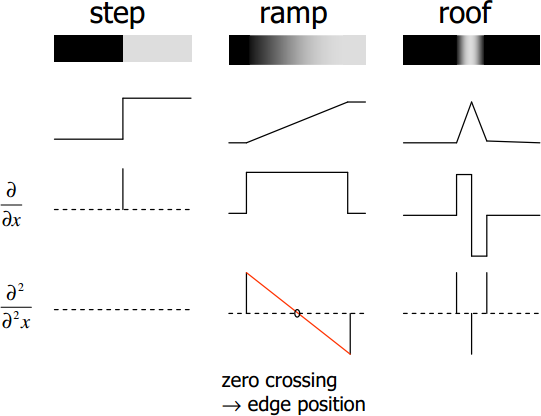
\includegraphics[width=5cm]{./images/derivatives.png}\\
  The second derivative is very sensible to noise (due to its highpass behaviour).
\end{minipage}

\clearpage
\skriptsection{Filtering in the Frequency Domain (V4)}{199}

\subsection{Discrete Fourier Transform (DFT)}
\begin{minipage}{11cm}
  \skriptsubsubsection{1-Dimensional}{220}
   $$s(h)=\sum_{k=0}^{N-1}\hat c_k e^{jhk\frac{2\pi}{N}}=
     \sum_{k=0}^{N-1} \left[ \hat{a}_k \cos\left(hk \frac{2 \pi}{N}\right)+\hat{b}_k \sin\left(hk
    \frac{2 \pi}{N}\right) \right]$$ with $N$ as the periodic number and the coefficients:\\
    $\hat{c}_k=\frac{1}{N} \sum\limits_{h=0}^{N-1}s(h) e^{-jhk\frac{2\pi}{N}}=\hat{a}_k-j\hat{b}_k = \Re\{c_k\} + j \Im\{c_k\}$ \\
    $\hat{a}_k=\frac{1}{N} \sum\limits_{h=0}^{N-1}s(h) \cos\left(hk \frac{2 \pi}{N}\right)=\Re\{\hat{c}_k\}$ \\
    $\hat{b}_k=\frac{1}{N} \sum\limits_{h=0}^{N-1}s(h) \sin\left(hk \frac{2 \pi}{N}\right)=-\Im\{\hat{c}_k\}$ 
  
  \skriptsubsubsection{2-Dimensional}{225}
    $$F(u,v) = \frac{1}{\sqrt{M N}} \sum_{x=0}^{N-1} \sum_{y=0}^{M-1} f(x,y) \exp\left( -j 2 \pi \left(\frac{ux}{M} + \frac{v y}{N} \right) \right)$$
\end{minipage}
\begin{minipage}{8cm}
  Beware, the Fast Fourier Transform is exactly the same as the DFT but faster.
  The phase contains important information and should not be discarded.\\
  
  To find out amplitude and phase:\\
  $|F(u,v)| = \sqrt{\Re\{F(u,v)\}^2 + \Im \{F(u,v)\}^2}$,\\
  $\varphi(u,v) = \arctan\left( \frac{\Im \{F(u,v)\}}{\Re\{F(u,v)\}} \right)$\\
  
  Examples of 2D-Fourier transform pairs \gonzales{243}.\\
  Fourier transform properties \gonzales{253f.}.\\
  
  In 2D, the DC values are visible at coordinates (0,0), but to better visualize the spectrum they 
  are usually moved to the center \matlab{fftshift}.  
\end{minipage}

\begin{minipage}{8cm}

\subsection{Border Problems}
  Due to the periodicity of the Fourier transform, borders are reproduced when no measures are taken.
  
  $F(k+N) = \sum\limits_{n=0}^{N-1} x_n e^{-\frac{2\pi j}{N} (k+N) n}$\\
  $=\sum\limits_{n=0}^{N-1} x_n e^{-\frac{2\pi j}{N} k n}  \underbrace{e^{-2 \pi j n}}_{1} = 
    \sum\limits_{n=0}^{N-1} x_n e^{-\frac{2\pi j}{N} k n} = F(k)$

\subsubsection{Padding}
  One way to avoid border problems is padding the original input image.
  
  From p. 263:
  \begin{aufzaehlung}
    \item Obtain padding parameters from input image $f(x,y)$ of size $M$x$N$. The padding parameters are 
    $P = 2M$ and $Q = 2N$
    \item Append zeros to input image to obtain the padded image $f_p(x,y)$
    \item Center its transform:\\
      $f_c(x,y) = f_p(x,y) \cdot (-1)^{x+y}$
    \item Compute DFT:\\
      $f_c(x,y) \FT F(u,v)$
    \item Filter:\\
      $F_f = F(u,v) \cdot H(u,v)$
    \item Compute IDFT:\\
      $F(u,v) \IFT g_p(x,y)$
    \item Extract original region $M$x$N$ from $g_p(x,y)$
  \end{aufzaehlung}
\end{minipage}
\begin{minipage}{11cm}
  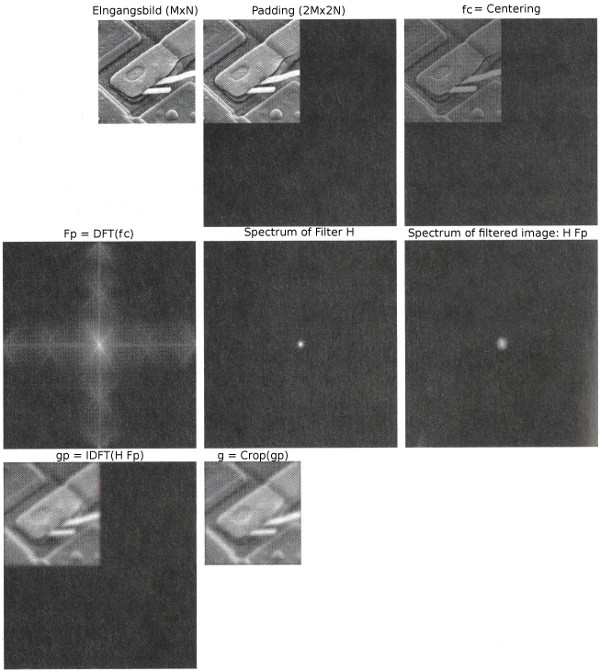
\includegraphics[width=11cm]{./images/frequency_filtering_padding.jpg}
\end{minipage}

\clearpage
\subsubsection{Window}
Another way is use windowing function which have nearly the size of the image and which smooth at 
the border to zero. In the spatial domain, they can be multiplied (which leads to convolution in 
the frequency domain).

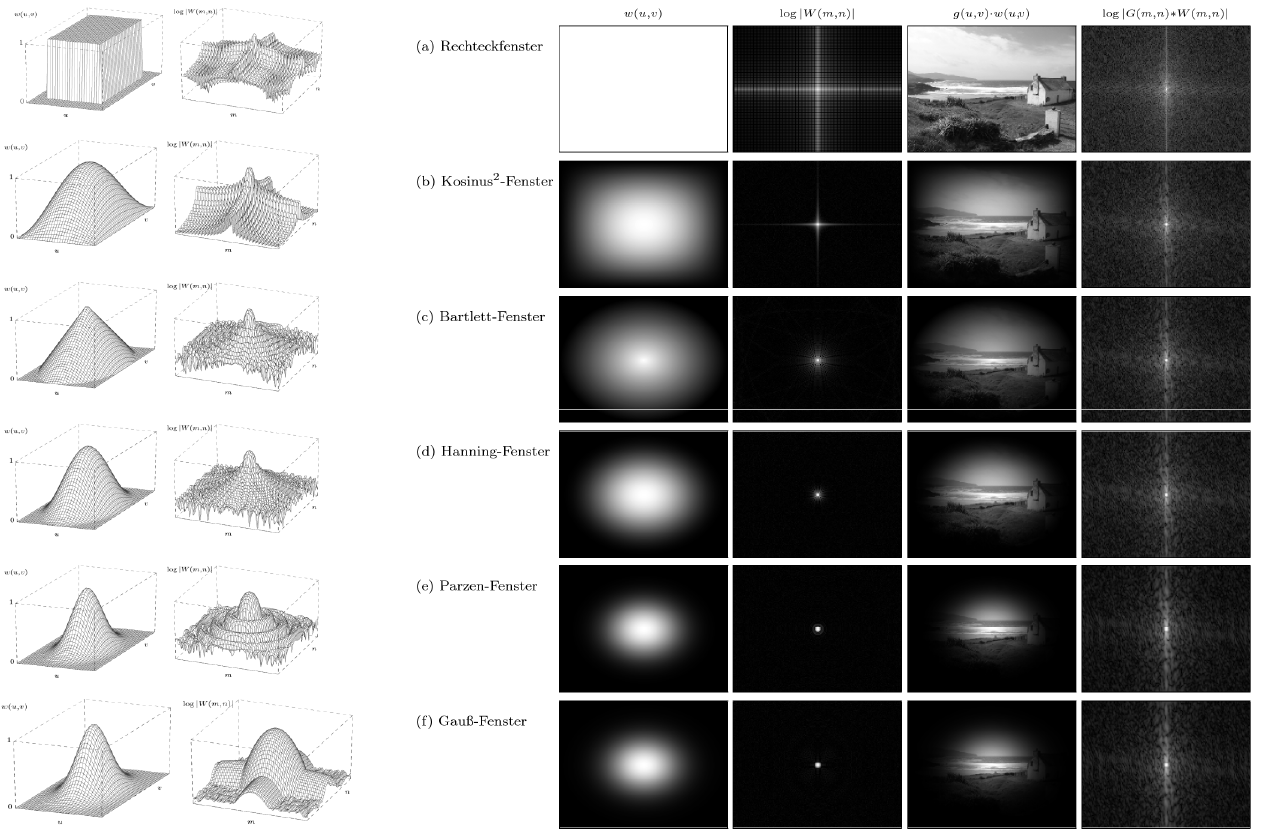
\includegraphics[width=\linewidth]{./images/window_functions.png}

\skriptsubsection{Filter Types}{269}
Filtering periodic noise can easily be done in the frequency domain.
E.g. band-rejection (notch) filter.\\
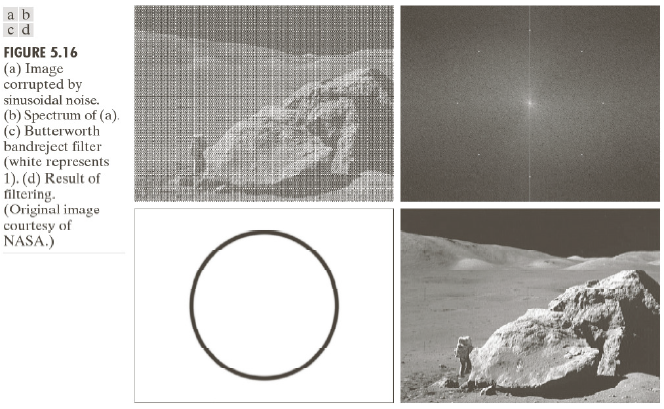
\includegraphics[width=10cm]{./images/periodic_noise_filter.png}
\skriptsection{Morphological Image Processing (V5, 6, 7)}{627}

  \skriptsubsection{Overview}{662}
  \begin{minipage}{9.5cm}
    Be aware of the $\hat{ }$ which is the reflection!\\
    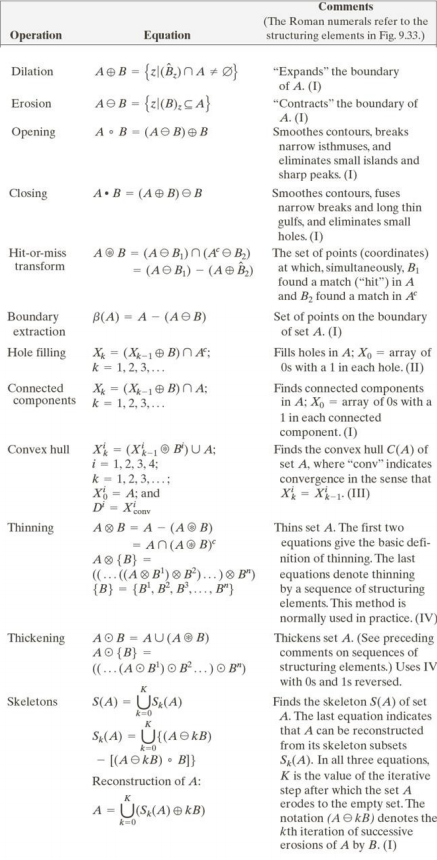
\includegraphics[width=9cm]{./images/morphology_table.png}
  \end{minipage}
  \begin{minipage}{9.5cm}
    Morphological approaches are nonlinear operations on binary or grey images.
    
    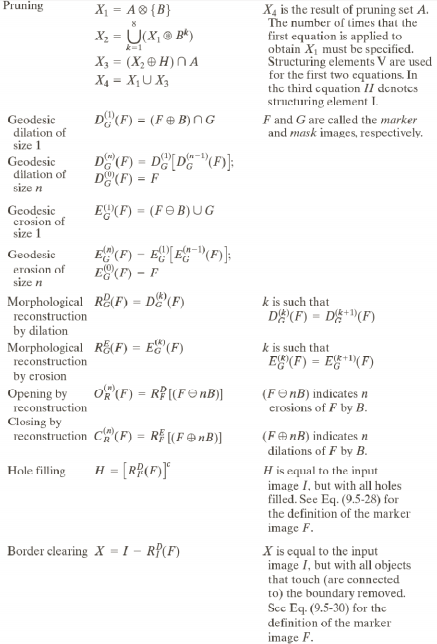
\includegraphics[width=9cm]{./images/morphology_table2.png}   
  \end{minipage}

  \skriptsubsection{Dilation}{633}
  Dilation (dt. wachsen) grows or thickens objects in a binary image. The structure element $H$
  is replicated at every foreground pixel of $I$:\\
  \begin{minipage}{9cm}
    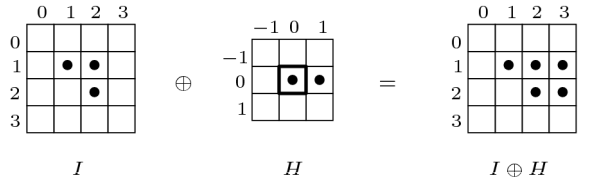
\includegraphics[width=9cm]{./images/dilatation.png}
  \end{minipage}
  \hspace{0.5cm}
  \begin{minipage}{9cm}
    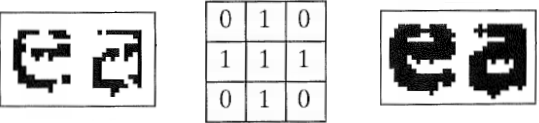
\includegraphics[width=9cm]{./images/dilatation_example.png}
  \end{minipage}
  
  \begin{minipage}{9.5cm}
    \subsubsection{Properties}
    \begin{liste}
      \item $I \oplus H = H \oplus I$
      \item $(I_1 \oplus I_2) \oplus I_3 = I_1 \oplus (I_2 \oplus I_3)$
      \item $I \oplus \delta = \delta \oplus I = I$ ($\delta$ is a neutral object)
    \end{liste}
  \end{minipage}
  \begin{minipage}{9.5cm}
    \subsubsection{Border conditions}
      It is best, to set the pixels at the border with the \textbf{minimum} value of $H$.
  \end{minipage} 

  \skriptsubsection{Erosion}{631}
  Erosion (dt. schrumpfen) shrinks or thins objects in a binary image. Only the pixels of the 
  original image where the structure element is completely encapseled, are in the resulting image.\\
  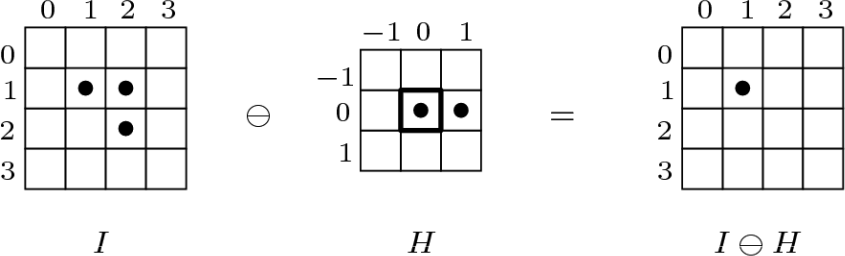
\includegraphics[width=9cm]{./images/erosion.png} 
  \hspace{0.5cm}
  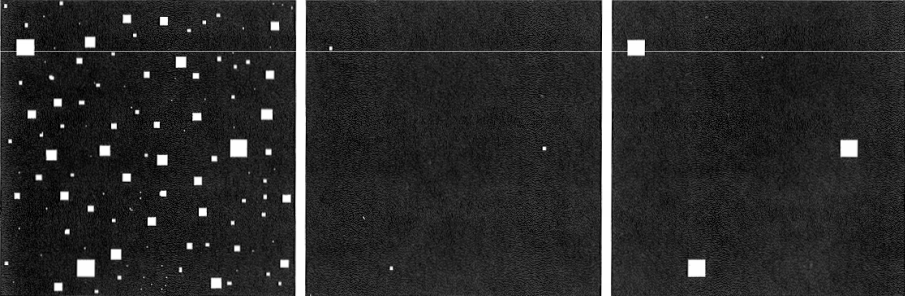
\includegraphics[width=9.5cm]{./images/erosion_example.png}
  \begin{minipage}{9.5cm}
    \subsubsection{Properties}
    \begin{liste}
      \item $I \ominus H \neq H \ominus I$
      \item $(I_1 \ominus I_2) \ominus I_3 \neq I_1 \ominus (I_2 \ominus I_3)$
    \end{liste}
  \end{minipage}
  \begin{minipage}{9.5cm}
    \subsubsection{Border conditions}
      It is best, to set the pixels at the border with the \textbf{maximum} value of $H$.
  \end{minipage}
  
  
  \skriptsubsection{Duality of Erosion and Dilation}{635}
  $(A \ominus B)^c = A^c \oplus \hat{B}$ \qquad
  $(A \oplus B)^c = A^c \ominus \hat{B}$ \qquad with $A^C$ being the complement of $A$ (binary inversion)
  
  
  \begin{minipage}{10cm}
    \skriptsubsection{Opening and Closing}{635}  
      \textbf{Opening}: $A \circ B = (A \ominus B) \oplus B$\\
      Foreground structures which are smaller than $H$ are eliminated by erosion. Dilation lets the
      structures grow back to its original size.  
      
    \textbf{Closing}: $A \bullet B = (A \oplus B) \ominus B$\\
      Holes in the foreground structures are eliminated by dilation. Erosion lets the
      structures shrink back to its original size.
      
    \textbf{Duality}: $(A \bullet B)^c = A^c \circ \hat{B})$, $(A \circ B)^c = A^c \bullet \hat{B})$
    
    \textbf{Properties}:
    \begin{liste}
      \item $A \circ B$, $A \bullet B$ are subsets of $A$
      \item $(A \circ B) \circ B = A \circ B$,  $(A \bullet B) \bullet B = A \bullet B$
    \end{liste}
  \end{minipage}
  \begin{minipage}{9cm}
    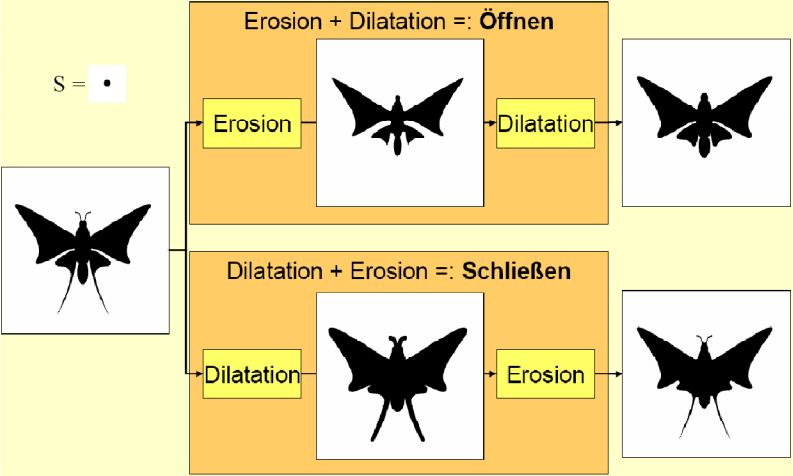
\includegraphics[width=9cm]{./images/morphology_opening_closing.png}
  \end{minipage}
  
  \vspace{1em}
  \begin{minipage}{9.2cm}
    \skriptsubsection{Hit-or-Miss Transform}{640}
      Finds shapes that are bigger than some (small) structure element $D$ and smaller than some 
      (big) second structure element $W$: $A \circledast B = (A \ominus D) \cap (A^c \ominus (W-D))$.
  \end{minipage}
  \hspace{0.6cm}
  \begin{minipage}{9.2cm}
    \skriptsubsection{Boundary Extraction}{642}
      Find difference between original image $A$ and erosion of $A$ with $B$: 
      $\beta(A) = A - (A \ominus B)$.
  \end{minipage}
  
  \vspace{1em}
  \begin{minipage}{9.2cm}
    \skriptsubsection{Hole Filling}{643}
      Fills out any holes (background regions) starting from a starting point: 
      $X_k = (X_{k-1} \oplus B) \cap A^c$ with $X_0$ being an image of same size as $A$ with single 
      pixels as starting point. This is an iterative approach.
      
      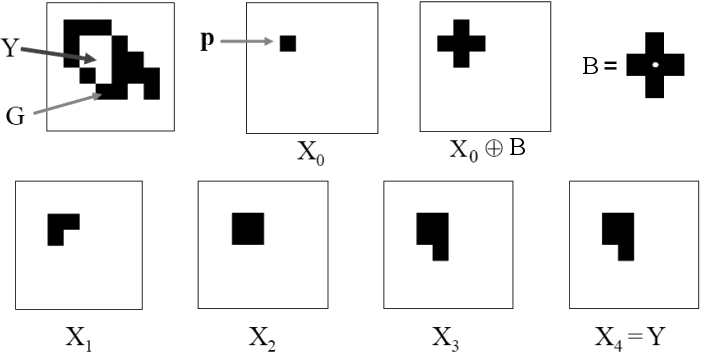
\includegraphics[width=7cm]{./images/morphology_hole_filling.png}
  \end{minipage}
  \hspace{0.6cm}
  \begin{minipage}{9.2cm}
    \skriptsubsection{Connected Components}{645}
      Find objects which are connected: $X_k = (X_{k-1} \oplus B) \cap A$.
      The only difference to hole filling is that here we are looking for foreground pixels instead of
      background pixels.
      \begin{flushright}
        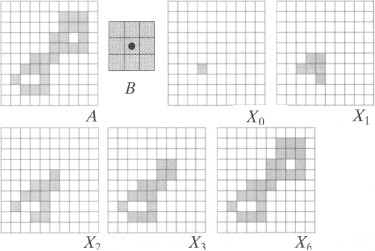
\includegraphics[width=5.5cm]{./images/morphology_connected_components.jpg}
      \end{flushright}
  \end{minipage}
  
  \begin{minipage}{11.5cm}
    \subsection{Other Tools} 
      Convex Hull \formelbuch{647}, Thinning \formelbuch{649}, Thickening \formelbuch{650}, 
      Skeletons \formelbuch{651}, Pruning \formelbuch{654}
      
    \skriptsubsection{Morphological Reconstruction}{656,676}
      Used after opening to grow back pieces of the original image that are connected to the opening.
      
      In addition to the structure element $B$ (block), here a marker image $F$ with starting points and a 
      mask image $G$ are required. $F \subseteq G$. 
  \end{minipage}
  \hspace{0.5cm}
  \begin{minipage}{7cm}
    \begin{flushright}
      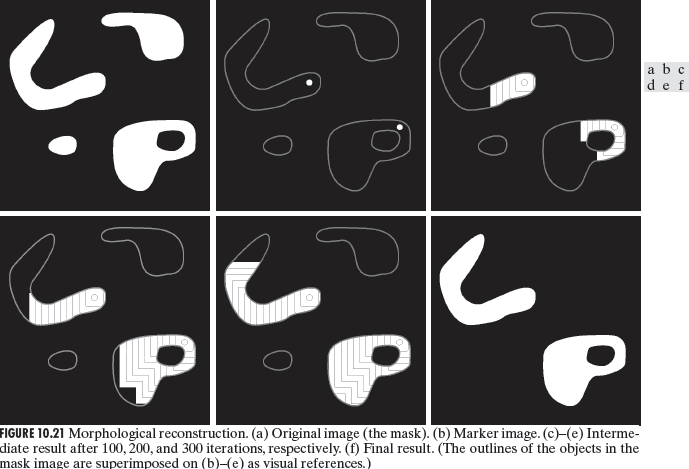
\includegraphics[width=7cm]{./images/morphology_reconstruction.png}
    \end{flushright}
  \end{minipage}
  \vspace{0.5em}
  
  \begin{minipage}{9.2cm}
    \skriptsubsubsection{Geodesic Dilation}{656}
      Init: $D_G^{(n)}(F)=F$ \\
      First it. (size 1): $D_G^{(1)}(F) = (F \oplus B) \cup G$\\
      Recursion (size $n$): $D_G^{(n)}(F) = D_G^{(1)}[D_G^{(n-1)}(F)]$
      
      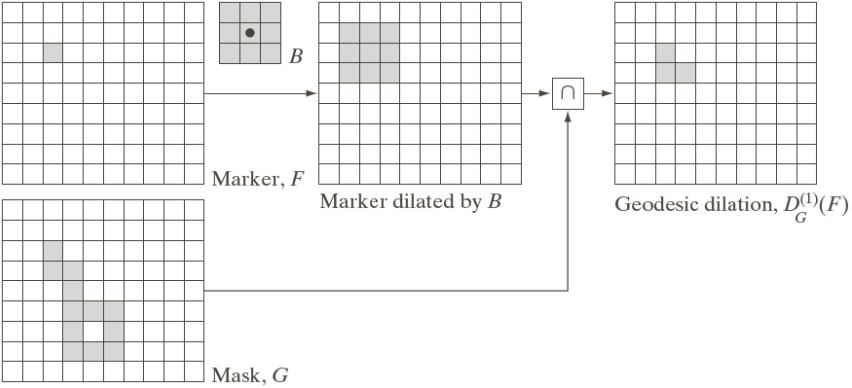
\includegraphics[width=8cm]{./images/morphology_geodesic_dilation.png}
      
    \skriptsubsubsection{Morphological Recon. by Dilation}{658}
      The iterative approach reconstructs the whole object out of a starting point.
      
      $R_G^D(F) = D_G^{(k)}(F)$
      
      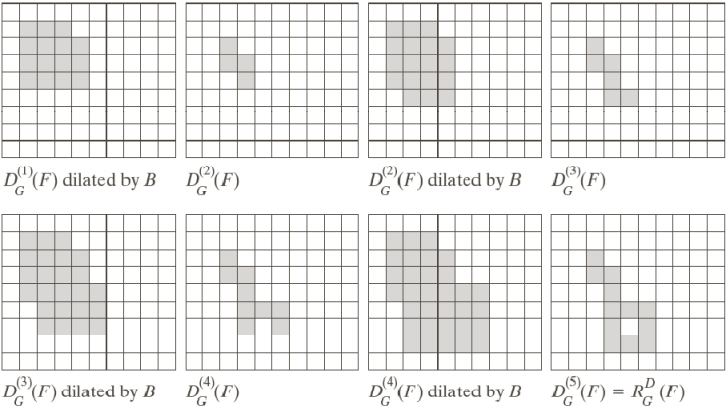
\includegraphics[width=8cm]{./images/morphology_reconstruction_dilation.png}
  \end{minipage}
  \begin{minipage}{9.2cm}
    \skriptsubsubsection{Geodesic Erosion}{657}
      Init: $E_G^{(n)}(F)=F$ \\
      First it. (size 1): $E_G^{(1)}(F) = (F \ominus B) \cap G$\\
      Recursion (size $n$): $E_G^{(n)}(F) = E_G^{(1)}[E_G^{(n-1)}(F)]$
        
      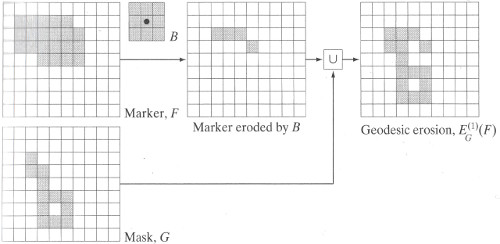
\includegraphics[width=8cm]{./images/morphology_geodesic_erosion.jpg}
      
    \skriptsubsubsection{Morphological Recon. by Erosion}{658}
      Reconstruction by erosion reconstructs holes.
      
      $R_G^E(F) = E_G^{(k)}(F)$
  \end{minipage}
  
  
  \skriptsubsubsection{Sample Applications}{659}
    \subsubsubsection{Opening by Reconstruction}
      Mask $g$ is the input image. The structure element $b$ can be selected to find meaningful starting 
      points (e.g. line with 50 pixels length).
      The marker is then calculated using $f = g \ominus b$.
      Then magic comes into play: The iterative reconstruction uses this equation: $(f \oplus nB) \bigwedge g$
      where $nB$ is the iteration number with 
      $0B = \begin{bmatrix}
      1&1&1\\
      1&1&1\\
      1&1&1\\
      \end{bmatrix}$
      and $\bigwedge$ is the minimum operator.
      This is done until the image is stable (does not change anymore).
      
    \subsubsubsection{Hole Filling} Automatic filling of holes (including starting point seeking)
    
    \subsubsubsection{Border Cleaning} e.g. OCR: All characters which contact the border can be 
    removed
  
  \skriptsubsection{Gray-Scale Morphology}{665}
    Uses function theory instead of set theory (Mengenlehre).
    In particular, the Top-Hat transformation \formelbuch{672} is interesting for shading 
    correction.
\clearpage
\section{Segmentation (V8, V9)}
  Segmentation subdivides an image into its constituent (zusammengehörend) regions or object. 
  $\Rightarrow$ One of the most
  difficult tasks in ImPro. Usually, post processing is required to identify and potentially label
  objects.
  
  Problems: Uneven illumination, noise
  
  \skriptsubsection{Edge Based Segmentation}{692}
    Aim: Finding borders or lines of objects: Contours, similarity of adjacent pixels can be detected.
    
    3 Steps:
    \begin{aufzaehlung}
      \item Preprocessing \& smoothing: noise reduction, small object removal, intensity transformations
      \item Edge point detection: Edge pixel detection, derivatives in X,Y direction with 1st and/or 2nd order filters (Laplacian)
      \item Postprocessing (localize edges): thresholding, thinning, zero crossings of 2nd order derivative
    \end{aufzaehlung}
    
    \skriptsubsubsection{Line Detection}{697}
      See spatial filters (Section \ref{sec:filter_types}) for Laplacian Sobel, Prewitt, \ldots
       
    \skriptsubsubsection{Point detection}{696}
      Point detection: Use 2nd order derivation (Laplacian): 
      $\nabla^2 f(x,y) = \frac{\delta^2 f}{\delta x^2} + \frac{\delta^2f}{\delta y^2} = 
      \left(f(x+1,y)+f(x-1,y)-2f(x,y)\right) + \left(f(x,y+1)+f(x,y-1)-2f(x,y)\right)$
      $H_{3 \times 3} = \begin{bmatrix}
        1 & 1 & 1 \\
        1 & -8 & 1 \\
        1 & 1 & 1 \\
      \end{bmatrix}$
    
    \skriptsubsubsection{Marr-Hildreth Edge Detector}{714}
      Intensity changes are not
      independent of image scale and so their detection requires the use of operators of different
      sizes; and that a sudden intensity change will give rise to a peak or trough (Mulde) in the first 
      derivative or equivalently a zero crossing in the second derivative.
      
      The operator for smoothing and Laplacian is called \em Laplacian of a Gaussian (LoG) \em or \em Mexican hat\em:
      $\nabla^2G(x,y) = \left( \frac{x^2 + y^2 2\sigma^2}{\sigma^4} e^{-\frac{x^2+y^2}{2\sigma^2}} \right)$
      with $\sigma$ being the standard deviation of the image.
      
      The size of the filter ($n \times n$) should be an odd integer with $n > \ceil(6 \sigma)$.
     
      Discussion:
      \begin{liste}
      	\item Strong smoothing (sharp edges might be lost)
      	\item Mostly closed edges
      	\item Sensitive to noise
      	\item Post-processing (zero-cross detection) required
      \end{liste}
  
    \skriptsubsubsection{Canny Edge Detector}{714}
      Use first order derivative in both directions.
      
      \begin{aufzaehlung}
      	\item Smooth image with Gaussian
      	\item Compute gradient (Sobel, Prewitt, \ldots) in both directions
      	\item Non-maxima suppression to gradient magnitude image (alles was nicht max ist, unterdrücken)
      	\item Double thresholding:
      	  \begin{liste}
      	  	\item Pixels with $f(x,y) > T_1$ belong to edge (strong edge pixels)
      	  	\item Pixels with $T_1 > f(x,y) > T_2$ belong to edge when there is a strong edge pixel
      	  	in the $8\times 8$ neighbourhood (weak edge pixels)
      	  \end{liste}
      	\item If necessary, edge thinning
      \end{aufzaehlung}
      This algo is considerably slower but performs better than Marr-Hildreth.
      
    \skriptsubsubsection{Edge Linking and Boundary Detection}{725}
      Edges are going to be linked together as they are typically not connected.
      
      \subsubsubsection{Local Processing}
        \begin{aufzaehlung}
        	\item Compute gradient $\nabla f= \begin{bmatrix}g_x\\g_y\end{bmatrix}$ (Sobel, Prewitt,\ldots)
          \item Compute magnitude $M(x,y) = \sqrt{g_x^2+g_y^2} \approx |g_x| + |g_y|$ and angle $\varphi(x,y) = \arctan(g_y/g_x)$
        	\item Set neighbour pixel (8-connected neighbours) at $(s,t)$ of pixel $(x,y)$ as edge
        	pixel when $|M(s,t) - M(x,y)| \leq m_0$ and $|\varphi(s,t) - \varphi(x,y)| \leq \varphi_0$
        	\item If necessary: Thinning and remove single edge pixels
        \end{aufzaehlung}
        
      \subsubsubsection{Global Processing}
        Find lines instead of simple edges
        
      \subsubsubsection{Hough Transform}
        See later\ldots
        
      \subsubsubsection{Edge Linking}
    
  \skriptsubsection{Thresholding}{738}
    \skriptsubsubsection{Definitions}{738}
      \begin{liste}
      	\item Global threshold: One threshold depending on intensity $T = T(f(x,y))$
      	\item Local threshold: Threshold may also depend on neighbourhood (e.g. grey level average, variance, \ldots)
      	  $T = T(f(x,y), p(x,y))$
      	\item Dynamic or variable or adaptive threshold: Depending on position: $T = T(x,y, f(x,y))$
      	\item Hysteresis thresholding: 1. Global threshold with $T_H$, 2. Threshold in the 
      	$k$-connected (e.g. $k=4,8$) neighborhood of all pixels detected in (1) with lower threshold $T_L$.
      \end{liste}
      
      Problems of thresholding: Noise, illumination
      
    \skriptsubsubsection{Basic Method}{741}
      \begin{aufzaehlung}
      	\item Initial $T$ (e.g. middle point between 2 maxima)
      	\item Segment image with $T$ into $G_1 \leq T$, $G_2 > T$
      	\item Compute average intensity value $m_1$, $m_2$ in $G_1$, $G_2$
      	\item Compute new threshold value: $T = \frac12 (m_1 + m_2)$
      	\item Repeat steps 2..4 until the difference of the $T$s is smaller than a constant $\epsilon$
      \end{aufzaehlung}
  
    \skriptsubsubsection{Otsu's Method}{742}
      Statistical approach to find best threshold.
      \begin{aufzaehlung}
      	\item Compute the normalized histogram of the input image. Denote the components of the 
      	  histogram by $p_i$, $i=0,1,\ldots,L-1$.
      	\item Compute cumulative sums: $P(k) = \sum_{i=0}^k p(i)$ for $k=0,1,\ldots,L-1$
      	\item Compute cumulative means: $m(k) = \sum_{i=0}^k i p(i)$ for $k=0,1,\ldots,L-1$
      	\item Compute global intensity mean: $m_G = \sum_{i=0}^{L-1} i p(i)$
      	\item Compute between-class variance: $\sigma_B^2(k) = \frac{(m_G P_1(k) - m(k))^2}{P_1(k)(1-P_1(k))}$ 
      	  for $k=0,1,\ldots,L-1$
      	\item Obtain Otsu threshold $k^* = \max_{k = 0,1,\ldots,L-1} \sigma_B^2(k)$. If max is not unique,
      	  average these $k$s.
      \end{aufzaehlung}
      Otsu is not always better than basic approach!
      
    \skriptsubsubsection{Smoothing}{747}
      Again, smoothing might improve results when noise is a problem.
      
    \skriptsubsubsection{Edges}{749}
      Improving the shape of histograms by considering only thoe pixels that lie on or near the edges
      between the objects and the background. $\Rightarrow$ less dependency of size of objects and background.
      \begin{aufzaehlung}
      	\item Find edges
      	\item Threshold edge image $\rightarrow$ binary image
      	\item Mask original image with thresholded edge image
      	\item Compute the histogram using only the pixels in the origianl image that correspond to 
      	  the locations of the 1-valued pixels in image from step 3. Evaluate threshold with the 
      	  basic method, Otsu, etc.
        \item Segment original image using this threshold
      \end{aufzaehlung}
      
    \skriptsubsubsection{Adaptive Thresholding}{756}
      \begin{tabular}{ll}
        \parbox{13cm}{
          Subdivide image and compute threshold for every region. Hint: 
          Regions must consist of both object and background, otherwise the thresholding would not 
          work and only distinguish between noise. Therefore, regions must be not too big and not too small.
      
    \skriptsubsubsection{Multivariable Thresholds}{761} 
      Use RGB color information for thresholding: $\bm z = [r, g, b]^T$. This is a 3D vector which 
      can also be referred as \em voxel \em (volume element).
      }
        & \parbox{6cm}{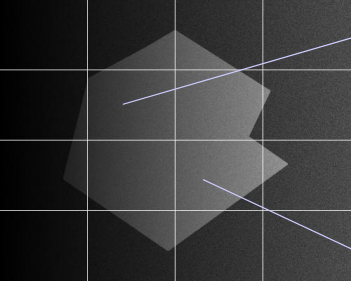
\includegraphics[width=5cm]{./images/adaptive_thresholding.png}}
      \end{tabular}

  \skriptsubsection{Region Based Segmentation}{763}
    Find boundaries between regions directly (in contrast to thresholding) according to some
    criteria (gray level, color, texture, form, \ldots). This is more efficient in terms of noisy
    and blurred images.
  
    \skriptsubsubsection{Region Growing}{763}
      \begin{enumerate}
      	\item Find seed points in input image $f(x,y)$ (e.g. with a very high threshold): $S(x,y)$
      	\item Morphological erosion of $S(x,y)$ to reduce connected components to 1 pixel
      	\item Calculate predicate: E.g. similarity in intensity (intensity threshold) on $f(x,y)$. 
      	  This leads to $f_Q(x,y)$ \todo{check}
      	\item Append found values to seed image and label every connected area.
      \end{enumerate}
      Starting with seed points, grow regions according to some ``criteria'' as mentioned above.
    
    
    \skriptsubsubsection{Splitting and Merging}{766}
      Instead of growing regions from seed points, this strategy grows from arbitrary disjoint regions.
      
      \begin{enumerate}
      	\item Split into four disjoint quadrants any region $R_i$ for which $Q(R_i)=FALSE$ ($Q(R_i)$ 
      	  is the predicate, pixels belonging to object)
      	\item Split all regions again into disjoint regions (if possible)
      	\item End splitting when no more splitting is possible
      \end{enumerate}
    
    \skriptsubsection{Watersheds}{769}
    \begin{minipage}{4cm}
      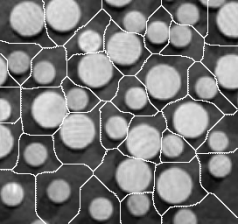
\includegraphics[width=4cm]{./images/morphology_watersheds.png}
    \end{minipage}
    \hspace{0.5cm}
    \begin{minipage}{14.5cm}
      The image can be viewed as a 3D relief with local minima. When ``flooding'' from these minima
      step by step and the ``water'' merges between two regions, a ``dam'' (Damm) can be built. These
      dams (watersheds/Wasserscheiden) are the dividers between regions.
      \begin{liste}
      	\item Use when uniform regions are searched
      	\item Problems: Oversegmentation due to noise or non-uniform regions.
      	\item Possible solutions:
          \begin{liste}
          	\item Smoothing (as always) but with relatively large kernels
          	\item Apply watershed transformation to gradient image (often still oversegmentation $\Rightarrow$ smoothing)
          	\item Use markers as starting point (e.g. shortest distance between black and white pixels)
          \end{liste}
      \end{liste}
    \end{minipage}
      
      
\skriptsection{Description and Representation (V10, 11, 12)}{795}
  \skriptsubsection{Representation}{796}
    A region can be represented in terms of its external characteristics (its boundary - basically for shape properties) or
    its internal characteristics (pixels comprising the region - basically for regional properties (colors, texture)).
    
    Description is the extraction of information out of the representation. For example the length
    of a boundary.
    
    These are some basic methods: Chain Codes \formelbuch{798}, Polygonal Approximations 
    \formelbuch{801} and Skeletons \formelbuch{812}.
    
    \begin{tabular}{ll}
      \parbox{10cm}{
        \skriptsubsubsection{Signatures}{808}
          Signature: 1d representation of a boundary that can be generated in various ways.
          
          Example: Distance from the centroid to the boundary as a function of angle:\\
          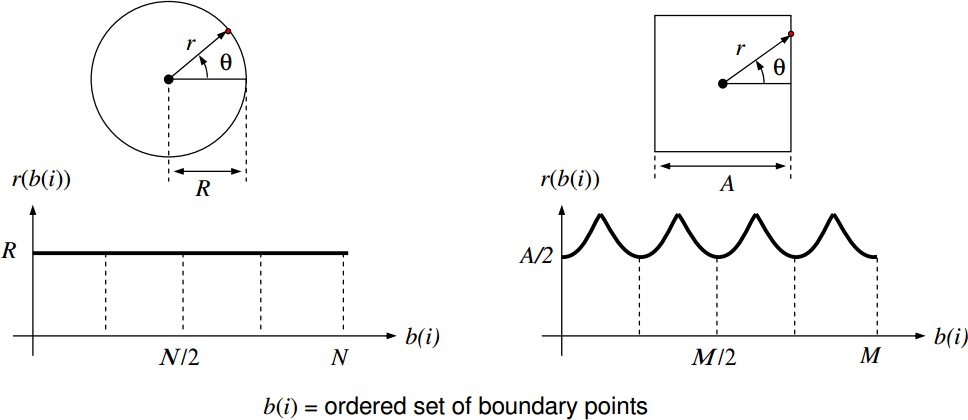
\includegraphics[width=9cm]{./images/signature.png}
          
          This signature generation is translation variant but not rotation or scaling variant.
          
          Features that can be used further are e.g. the number of maxima or the distance between maximum and minimum.}
      & \parbox{9cm}{
          \skriptsubsubsection{Fourier Descriptors}{818}
            FDs represent the frequency content of a shape (of the border) which can also be viewed as the form of an object.
            It is possible to make them independent of various transformations:\\
            \begin{tabular}{ll}
              Translation & $F(0) = 0$\\
              Scale & $F(u) = \frac{F(u)}{|F(1)|}$\\
              Rotation, starting point , direction & $F(u) = |F(u)|$ 
            \end{tabular}
            FDs are insensitive to noise.
            
            However, this might be dangerous as information (phase) is thrown away and may lead to wrong assumptions:\\
            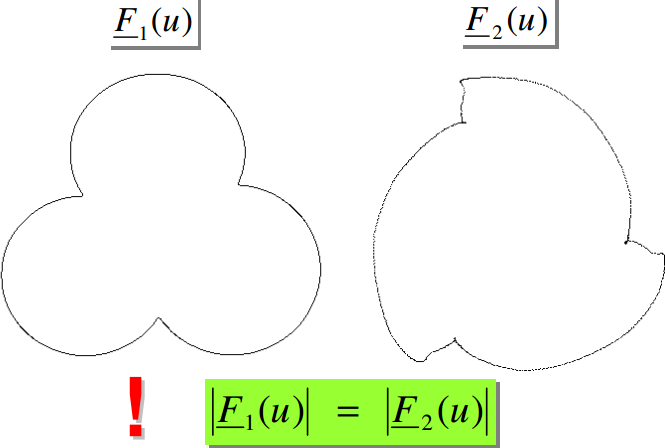
\includegraphics[width=5cm]{./images/fourier_descriptiors_danger.png}
            }
    \end{tabular}
      
      
    
    \skriptsubsubsection{Hough Transform (HT)}{735}
      Aim: Find lines, circles or any freeform shapes in an image after edge detection.
      
      \subsubsubsection{HT for Lines}
      The objects are found using the following algorithm:\\
      \begin{tabular}{|l|l|}
        \hline
        \textbf{Step} & \textbf{Example: Line} \\
        \hline
        Define mathematical equation which describes the shape.
          & $y = a_k x + b_k$ \\
        \hline
        Define parameter space with limits
          & $a_k \in [a_{min}, a_{max}]$, $b_k \in [b_{min}, b_{max}]$ \\
        \hline
        \parbox{9cm}{For every point $x_i$, $y_i$ solve $b = y_i-ax_i$ and increment each visited 
          point: $H(a,b)=H(a,b)+1$ \todo{check}}
          & \parbox{9cm}{
            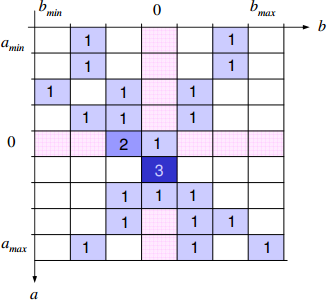
\includegraphics[width=6cm]{./images/hough_transform_parameterspace.png}
            } \\
        \hline
        Find maximum value in parameter space
          & Marked deep blue in graphics above (with 3 in it) \\
        \hline
        Parameters inserted into equation leads to most likely object
          & $y = a x + b$ \\
        \hline
      \end{tabular}
      
      Problem with this is that a horizontal line leads to $a \rightarrow \infty$. Therefore,
      the parameter equation $x \cos(\Theta) +  \sin(\Theta) = r$ should be used for finding
      a line.
      
      \subsubsubsection{Equations for circles}\\
      \begin{tabular}{lll}
        \parbox{8cm}{Cartesian equation:\\
           $r^2 = (x-x_0)^2 + (y-y_0)^2$ \\ \\
           Parametric representation:\\
           $x=x_0 + r \cos(\Theta)$\\
           $y=y_0+r\cos(\Theta)$\\
           with $\Theta$ not being a free parameter}
          & \parbox{5cm}{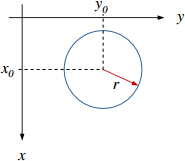
\includegraphics[width=4cm]{./images/hough_transform_circle.png}}
          & \parbox{5cm}{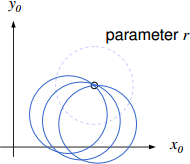
\includegraphics[width=4cm]{./images/hough_transform_circle2.png}}
      \end{tabular}
      
      
      \subsubsubsection{Generalized Hough Transform (GHT)}\\
        For freeform shapes which are rotation and scaling invariant as well as some a priori 
        knowledge of the shape is available.
        Here, the \em gradient of the boundary \em is used instead of a parameter model. The space is now called \em reference
        space \em and not parameter space anymore.
        
      \subsubsubsection{Conclusions}
        \begin{liste}
        	\item Quite high computational effort (``Brute Force''), but control by quantization of parameter space
        	\item Multiple objects can be detected
        	\item HT tolerates also objects with ``holes'' 
        \end{liste}
    
    \subsubsection{Harris Corner Detection}
      \begin{tabular}{ll}
        \parbox{13cm}{
          Corners are reference landmarks in images and help in localization.
          A corner has two large eigenvalues in the structure tensor $T_s$.
          
          \begin{aufzaehlung}
            \item  if necessary (eg. noise, etc.) low-pass filter the image 
            \item  compute gradients $G_x$, $G_y$ (sobel)
            \item  build the structure tensor: 4 (3) values per pixel
            \item  low-pass filter each component of the structure tensor
            \item  compute Harris corner measure $R(x,y)$ from structure tensor
            \item  threshold $R(x,y)$ with $T_th > 0 \rightarrow$ potential corners
            \item  use non-maxima suppression to find maxima in $R(x,y)$
              \begin{liste}
                \item sort maxima in descending order
                \item select largest maximum
                \item suppress maxima within radius $r$ around selected maximum
                \item select remaining largest maximum
                \item ... etc
              \end{liste}
          \end{aufzaehlung}
          }
          & \parbox{5cm}{
            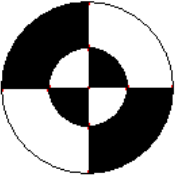
\includegraphics[width=4cm]{./images/marker.png}}
      \end{tabular}
      

  \clearpage
  \begin{minipage}{9cm}
  \skriptsubsection{Simple Descriptors}{822}
    Simple descriptors include area, perimeter, minimum/maximum diameter, area of bounding rectangle and
    should be independent of translation, rotation and scale.
     
    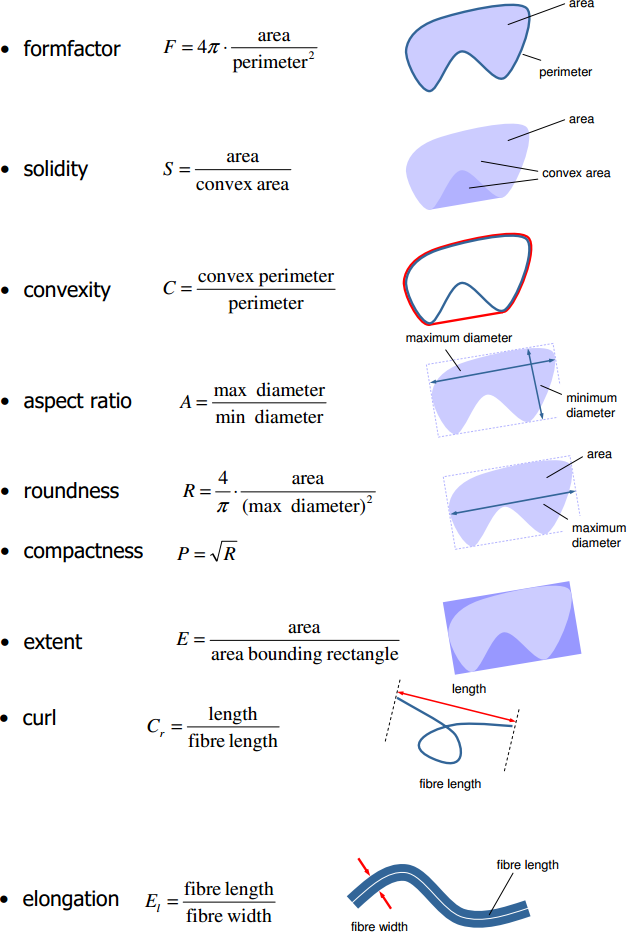
\includegraphics[width=8cm]{./images/simple_descriptors.png}
    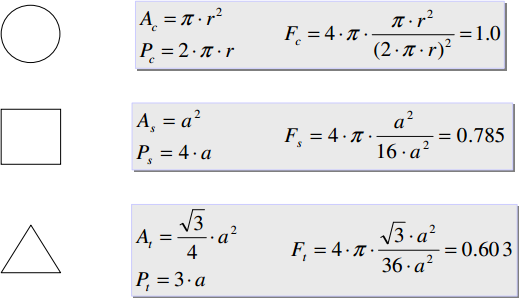
\includegraphics[width=8cm]{./images/simple_descriptors_formfactors.png}
    
    
    \skriptsubsection{Area Based Descriptors (Moments)}{839}
      Moments are statistical measures of the shape of a set of points. Due to its statistical
      nature, they are hardly variant to translation, rotation and scale.
      
      2D moments of order $p+q$: $$m_{pq} = \sum_{x=0}^{M-1} \sum_{y=0}^{N-1} x^p y^p f(x,y)$$
      
  \end{minipage}
  \begin{minipage}{9cm}
    \textbf{Area based descriptors, continued}
    
      2D \em central \em moments of order $p+q$: $$\mu_{pq} = \sum_{x=0}^{M-1} \sum_{y=0}^{N-1} (x-\bar{x})^p (y-\bar{y})^p f(x,y)$$
      with $\bar{x}=\frac{m_{10}}{m_{00}}$ and $\bar{y}=\frac{m_{01}}{m_{00}}$ which are also the
      centroid coordinates.
      
      Use principal components for normalizing with respect to variations in size, translation and 
      rotation.
      
      Moments provide:
      \begin{compactList}
        \item Centroid coordinates
        \item Principal axes of inertia (Trägheit) or direction of maximal and minimal 
          variance (principal components)
        \item Minimal bounding box
      \end{compactList}
    
    \skriptsubsection{Texture Based Descriptors}{827}
      \subsubsection{Statistical Approaches}
        Based on normalized histogram $h(g)$ (global):\\ 
        \begin{compactList}
          \item Mean: $m=\sum_{i=0}^{L-1} g_i h(g_i)$
          \item Variance: $\mu_2 = \sigma^2 = \sum_{i=0}^{L-1} (g_i-m)^2 h(g_i)$
          \item Skewness: $\mu_3 = \sum_{i=0}^{L-1} (g_i-m)^3 h(g_i)$
          \item Roughness: $R(g) = 1 - \frac{1}{1 + \sigma^2/(L-1)^2}$\\
            $R \rightarrow 1$: large $\sigma$, rough; $R \rightarrow 0$: $\sigma = 0$, smooth
          \item Uniformity (uniformity): $U(g) = \sum_{i=0}^{L-1} h^2(g_i)$
          \item Average entropy: \\$H(g) = -\sum_{i=0}^{L-1} h(g_i) \log_2(h(g_i))$
        \end{compactList}
      
      \subsubsection{Co-Occurence Matrix}
        The construction of COO uses the following scheme, it is local: \\
        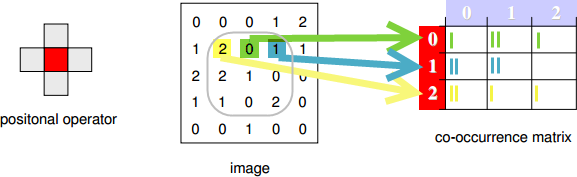
\includegraphics[width=8cm]{./images/cooccurence_matrix.png} \\
        The row index indicates the value of the center
        and the columns the number of values in the PO.
        
        The COO can also be reduced (instead of 255 grey intensities only 64 or 8 could be evaluated).
        
        \begin{tabular}{ll}
          Energy
            & $E = \sum_{i=0}^{L-1} \sum_{j=0}^{L-1} COO(i,j)^2$ \\
          Contrast
            & $C = \sum_{i=0}^{L-1} \sum_{j=0}^{L-1} (i-j)^2 COO(i,j)$ \\
          Entropy
            & $H = \sum_{i=0}^{L-1} \sum_{j=0}^{L-1} COO(i,j) \log(COO(i,j))$ \\
          Homogenity
            & $S = \sum_{i=0}^{L-1} \sum_{j=0}^{L-1} \frac{COO(i,j)}{1+|i-j|}$ \\
        \end{tabular}
        
    \subsubsection{Spectral Approach}
      Energy, contrast, entropy can also be found out using the scaled spectrum:
      $$S(u,v) = FFT(f(x,y)) \qquad S_n(u,v) = \frac{|S(u,v)}{\sqrt{\sum\limits_{u=2}^{m} \sum\limits_{v=2}^n |S(u,v)|}}$$
  \end{minipage}
    
    
\skriptsection{Object Recognition V13, 14}{861}
  \begin{minipage}{8cm}
    Problems: Which features are to be used? Where are the boundaries?
    
    Definition of a pattern or feature vector: \\
    $\bm x = [x_1, \ldots, x_n]^T$
    Classes: $\bm x \rightarrow K_1, \ldots, K_W$
  
    \subsection{Decision Theory}
        
      \skriptsubsubsection{Minimum Distance Classification}{866}
        Sample will be assigned to the class to which the mean is the shortest. 
        
        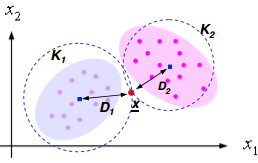
\includegraphics[width=5cm]{./images/minimum_distance_classifier.png}
        
        When the \em Mahalanobis distance \em is taken instead of the Euclidean distance, the variance is 
        also included in the min-dist-classifier:
        $$\boxed{D_j(\bm{x})^2 = (\bm x - \bm m_j)^T \bm{C}_j^{-1} (\bm x -\bm m_j)}$$
        with $\bm C_j$ as the covariance matrix for every 
        sample per class: 
        $$\bm C_j = \frac{1}{N_j} \sum_{\bm x \in K_j} \bm x \bm x^T - \bm m_j \bm m_j^T.$$
        
      \skriptsubsubsection{Matching by Correlation}{869}
        Correlation is not robust in terms of background and freeform objects (only square objects).
        
      \skriptsubsubsection{Bayes Classifier}{874}
        Binary loss function: $d_j(\bm x) = p(\bm x | K_j) p(K_j)$ ($j=1,\ldots,W$).
        $p(\bm x | K_j)$ is assumed to be Gaussian distributed:      
        $$d_j(\bm x) = \ln p(K_j)  - \frac{1}{2} \ln |\bm C_j| - \frac12 (\bm x - m_j)^T \bm C_j^{-1} (\bm x - m_j)) $$
      
      
  \end{minipage} \hspace{5mm}
  \begin{minipage}{10cm}
  
    \skriptsubsection{Neural Nets}{882}
      No assumptions about statistical model, training via samples.
      
      2-Layer perceptron for linearly separable classes
      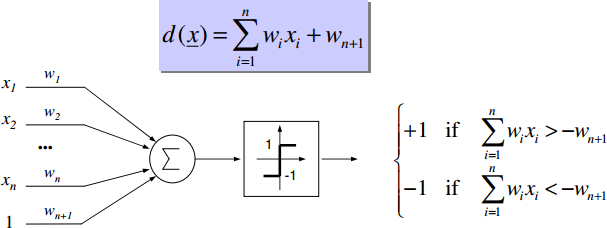
\includegraphics[width=6cm]{./images/2layer-perceptron.png}
      
      3-Layer perceptron for non-linearly separable classes with nonlinear perceptron function
      
      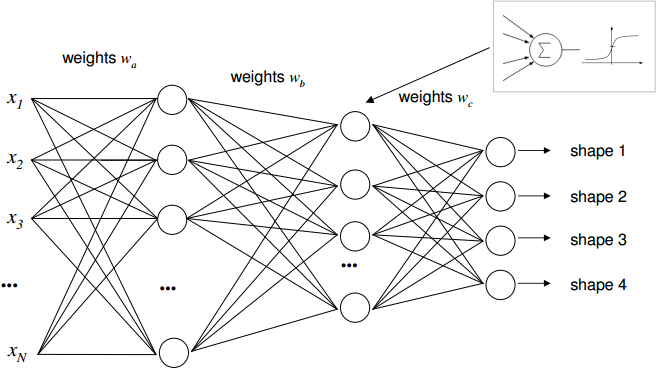
\includegraphics[width=6cm]{./images/multilayer-perceptron.png}
      
    \skriptsubsection{Structural Methods}{903}
      Classification based on common descriptors (order descriptors) according to degree of similarity:\\
      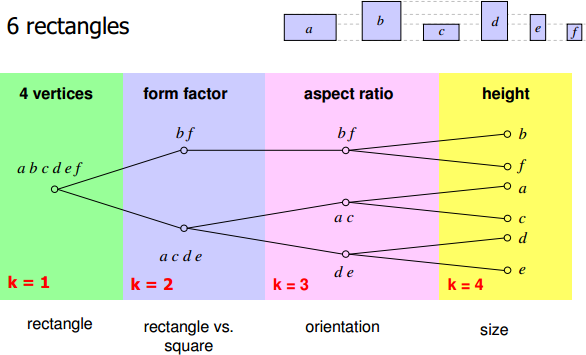
\includegraphics[width=7cm]{./images/common_features.png}\\
      Measure the similarity: Largest number to which $k$ is the same.
      Distance between two objects $a$ and $b$: $D(a,b) = \frac{1}{k}$
      
      Build similarity matrix:\\
      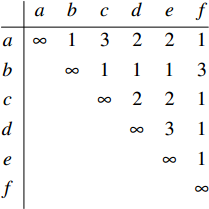
\includegraphics[width=3cm]{./images/similarity_matrix.png}
  \end{minipage}

  \skriptsubsection{Grammar}{904}
    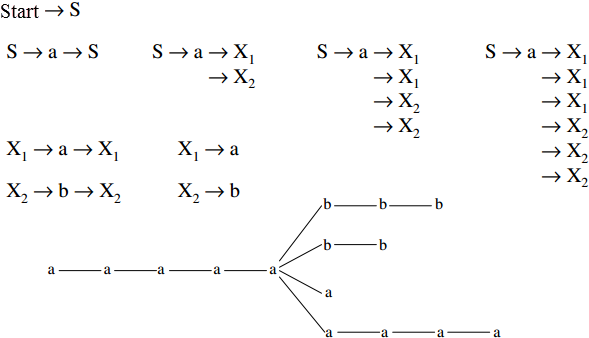
\includegraphics[width=7.5cm]{./images/grammar.png}
      

\end{document}
